\documentclass{article}

\usepackage{fancyhdr}
\usepackage{extramarks}
\usepackage{amsmath}
\usepackage{amsthm}
\usepackage{amssymb}
\usepackage{amsfonts}
\usepackage{tikz}
\usepackage[plain]{algorithm}
\usepackage{algpseudocode}
\usepackage{float} 
\usepackage{cancel}
\usepackage{algorithm}


\usetikzlibrary{automata,positioning}

%
% Basic Document Settings
%

\topmargin=-0.45in
\evensidemargin=0in
\oddsidemargin=0in
\textwidth=6.5in
\textheight=9.0in
\headsep=0.25in

\linespread{1.1}

\pagestyle{fancy}
\lhead{\hmwkAuthorName}
\chead{\hmwkClass\ \hmwkTitle}
%\chead{\hmwkClass\ (\hmwkClassInstructor\ \hmwkClassTime): \hmwkTitle}
\rhead{\firstxmark}
\lfoot{\lastxmark}
\cfoot{\thepage}

\renewcommand\headrulewidth{0.4pt}
\renewcommand\footrulewidth{0.4pt}

\setlength\parindent{0pt}

%
% Create Problem Sections
%

\newcommand{\enterProblemHeader}[1]{
    \nobreak\extramarks{}{Problem \arabic{#1} continued on next page\ldots}\nobreak{}
    \nobreak\extramarks{Problem \arabic{#1} (continued)}{Problem \arabic{#1} continued on next page\ldots}\nobreak{}
}

\newcommand{\exitProblemHeader}[1]{
    \nobreak\extramarks{Problem \arabic{#1} (continued)}{Problem \arabic{#1} continued on next page\ldots}\nobreak{}
    \stepcounter{#1}
    \nobreak\extramarks{Problem \arabic{#1}}{}\nobreak{}
}

\setcounter{secnumdepth}{0}
\newcounter{partCounter}
\newcounter{homeworkProblemCounter}
\setcounter{homeworkProblemCounter}{1}
\nobreak\extramarks{Problem \arabic{homeworkProblemCounter}}{}\nobreak{}

%
% Homework Problem Environment
%
% This environment takes an optional argument. When given, it will adjust the
% problem counter. This is useful for when the problems given for your
% assignment aren't sequential. See the last 3 problems of this template for an
% example.
%
\newenvironment{homeworkProblem}[1][-1]{
    \ifnum#1>0
        \setcounter{homeworkProblemCounter}{#1}
    \fi
    \section{Problem \arabic{homeworkProblemCounter}}
    \setcounter{partCounter}{1}
    \enterProblemHeader{homeworkProblemCounter}
}{
    \exitProblemHeader{homeworkProblemCounter}
}

%
% Homework Details
%   - Title
%   - Due date
%   - Class
%   - Section/Time
%   - Instructor
%   - Author
%

\newcommand{\hmwkTitle}{Homework\ \#4}
\newcommand{\hmwkDueDate}{March 17, 2022 (2 days free late.)}
\newcommand{\hmwkClass}{EECS 545 Machine Learning}
\newcommand{\hmwkClassTime}{Section A}
\newcommand{\hmwkClassInstructor}{Professor Honglak Lee}
\newcommand{\hmwkAuthorName}{\textbf{Yuang Huang}}
\newcommand{\hmwkUninameName}{\textbf{yahuang@umich.edu}}

%
% Title Page
%

\title{
    \vspace{2in}
    \textmd{\textbf{\hmwkClass:\ \hmwkTitle}}\\
    \normalsize\vspace{0.1in}\small{Due\ on\ \hmwkDueDate\ at 11:59pm}\\
    \vspace{0.1in}\large{\textit{\hmwkClassInstructor\ \hmwkClassTime}}
    \vspace{3in}
}

\author{\hmwkAuthorName\\
\hmwkUninameName}
\date{}

\renewcommand{\part}[1]{\textbf{\large Part \Alph{partCounter}}\stepcounter{partCounter}\\}

%
% Various Helper Commands
%

% Useful for algorithms
\newcommand{\alg}[1]{\textsc{\bfseries \footnotesize #1}}

% For derivatives
\newcommand{\deriv}[1]{\frac{\mathrm{d}}{\mathrm{d}x} (#1)}

% For partial derivatives
\newcommand{\pderiv}[2]{\frac{\partial}{\partial #1} (#2)}

% Integral dx
\newcommand{\dx}{\mathrm{d}x}

% Alias for the Solution section header
\newcommand{\solution}{\textbf{\large Solution}}

% Probability commands: Expectation, Variance, Covariance, Bias
\newcommand{\E}{\mathrm{E}}
\newcommand{\Var}{\mathrm{Var}}
\newcommand{\Cov}{\mathrm{Cov}}
\newcommand{\Bias}{\mathrm{Bias}}

\begin{document}

\maketitle

\pagebreak

\begin{homeworkProblem}
    \large {Neural Network Layer Implementation}
    \\
    \textbf{Solution}\\
    \textbf{Part a:}\\
    \begin{equation}
        \begin{aligned}
            \frac{\partial L}{\partial W_{ij}} &= \sum_{n = 1}^{N}\sum_{m=1}^{D_{out}} \frac{\partial L}{\partial Y_m^{n}} \frac{\partial Y_m^{n}}{\partial W_{ij}}\\
            Y = XW + B &\Rightarrow Y_m^n = \sum_{i=1}^{D_{out}} X_i^n W_{m,i} + b_m\\
            \Rightarrow \frac{\partial L}{\partial W_{ij}} &= \sum_{n=1}^N\frac{\partial L}{\partial Y_i^n} \frac{Y_i^n}{\partial W_{ij}}\\
            &= \sum_{n=1}^N\frac{\partial L}{\partial Y_i^n}X_j^n\\
            \Rightarrow \frac{\partial L}{\partial W} &= \mathbf{X}^T \frac{\partial L}{\partial Y} 
        \end{aligned}
    \end{equation}.\\

    \begin{equation}
        \begin{aligned}
            \frac{\partial L}{\partial b_{j}} &= \sum_{n = 1}^{N}\sum_{m=1}^{D_{out}} \frac{\partial L}{\partial Y_m^{n}} \frac{\partial Y_m^{n}}{\partial b_{j}}\\
            Y = XW + B &\Rightarrow Y_m^n = \sum_{i=1}^{D_{out}} X_i^n W_{m,i} + b_m\\
            \Rightarrow \frac{\partial L}{\partial b_{j}} &= \sum_{n=1}^N\frac{\partial L}{\partial Y_j^n} \frac{Y_j^n}{\partial b_{j}}\\
            &= \sum_{n=1}^N\frac{\partial L}{\partial Y_i^n} \cdot 1\\
            \Rightarrow \frac{\partial L}{\partial b} &= \sum_{n=1}^N\frac{\partial L}{\partial Y} 
        \end{aligned}
    \end{equation}.\\

    \begin{equation}
        \begin{aligned}
            \frac{\partial L}{\partial X_{i}^n} &= \sum_{n = 1}^{N}\sum_{m=1}^{D_{out}} \frac{\partial L}{\partial Y_m^{n}} \frac{\partial Y_m^{n}}{\partial X_{i}^n}\\
            Y = XW + B &\Rightarrow Y_m^n = \sum_{i=1}^{D_{out}} X_i^n W_{m,i} + b_m\\
            \Rightarrow \frac{\partial L}{\partial X_{i}^n} &= \sum_{n=1}^N\frac{\partial L}{\partial Y_i^n} \frac{Y_i^n}{\partial X_{i}^n}\\
            &= \sum_{m=1}^{D_{out}}\frac{\partial L}{\partial Y_m^n}W_{m,i}\\
            \Rightarrow \frac{\partial L}{\partial X} &= \frac{\partial L}{\partial Y} \mathbf{W}^T 
        \end{aligned}
    \end{equation}.\\
    \textbf{Part b:}\\
    Because
    \begin{equation}
        \frac{\partial Y}{\partial X}=\left\{
        \begin{array}{ll} 
        1, &x \geq 0 \\
        0, &x < 0
        \end{array}
        \right.
    \end{equation}

    \begin{equation}
        \frac{\partial L}{\partial X}=\frac{\partial L}{\partial Y}\frac{\partial Y}{\partial X} = \left\{
        \begin{array}{ll} 
        \frac{\partial L}{\partial Y}, &x \geq 0 \\
        0, &x < 0
        \end{array}
        \right.
    \end{equation}
    \textbf{Part c:}\\



\end{homeworkProblem}

\pagebreak

\begin{homeworkProblem}
    \large Multi-class classification with Softmaxs\\

    \textbf{Solution}

    \textbf{Part a:}\\
    
    \textbf{Part b:}\\

    \textbf{Part c:}\\
    $\bullet$ hidden-dim = 10 \\train acc = 0.937000 val acc = 0.951800 \\
    $\bullet$ hidden-dim = 50 \\train acc =  0.983000 val acc  = 0.972400  \\
    $\bullet$ hidden-dim = 100 \\ train acc = 0.985000 val acc = 0.977200  \\
    $\bullet$ hidden-dim = 250 \\ train acc = 0.985000 val acc = 0.978400  \\
    $\bullet$ hidden-dim = 500 \\ train acc = 0.988000 val acc = 0.981400  \\
    $\bullet$ hidden-dim = 800 \\ train acc = 0.988000 val acc = 0.983600   \\
    $\bullet$ hidden-dim = 1200 \\ train acc = 0.987000 val acc = 0.981400  \\
    $\bullet$ hidden-dim = 1600  \\ train acc = 0.990000 val acc = 0.982600 \\

    We will find that the best setting for thr number of hidden units based on the performance on validation set is hidden-dim = 800.
    \begin{figure}[H]  
        \centering  
        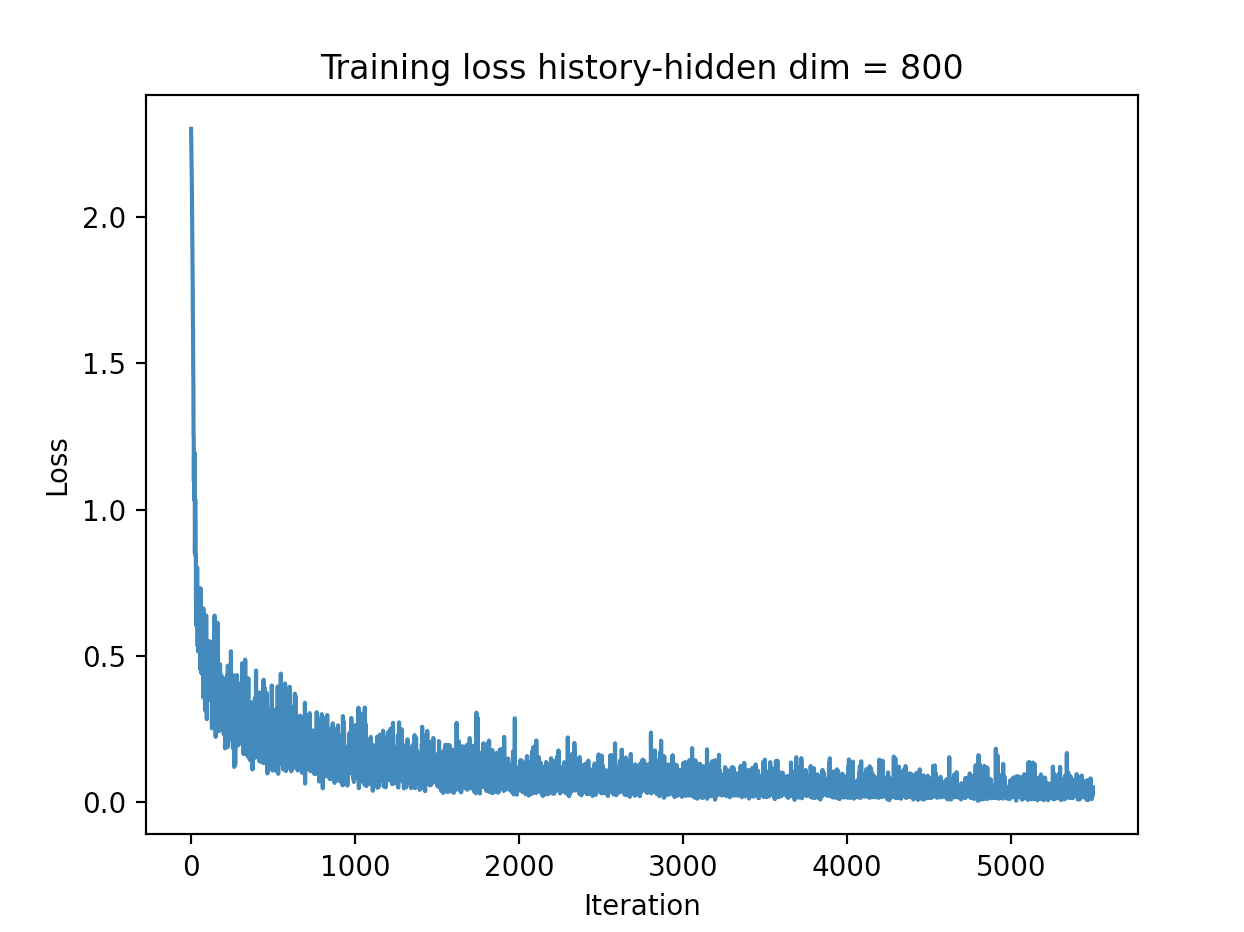
\includegraphics[width=4in,height=3.2in]{800} 
        \caption{Training loss history} 
    \end{figure}
    Figure 1 shows the training loss history where hidden-dim = 800. Using the optimal setting from 
    the previous step, train my network again, the accuracy obtained on the test set is 0.9793.

\end{homeworkProblem}

\pagebreak

\begin{homeworkProblem}
    \large Convolutional Neural Network for multi-class classification\\

    \textbf{Solution}

    \textbf{Part a:}\\

    \textbf{Part b:}\\

    \textbf{Part c:}\\
    The accuracy obtained on the test set is 0.9771 (hidden-dim = 100).
\end{homeworkProblem}

\pagebreak

\begin{homeworkProblem}
    \large Convolutional Neural Network for multi-class classification\\

    \textbf{Solution}

    \textbf{Part a:}\\

    \textbf{Part b:}\\

    \textbf{Part c:}\\
    \begin{figure}[H]  
        \centering  
        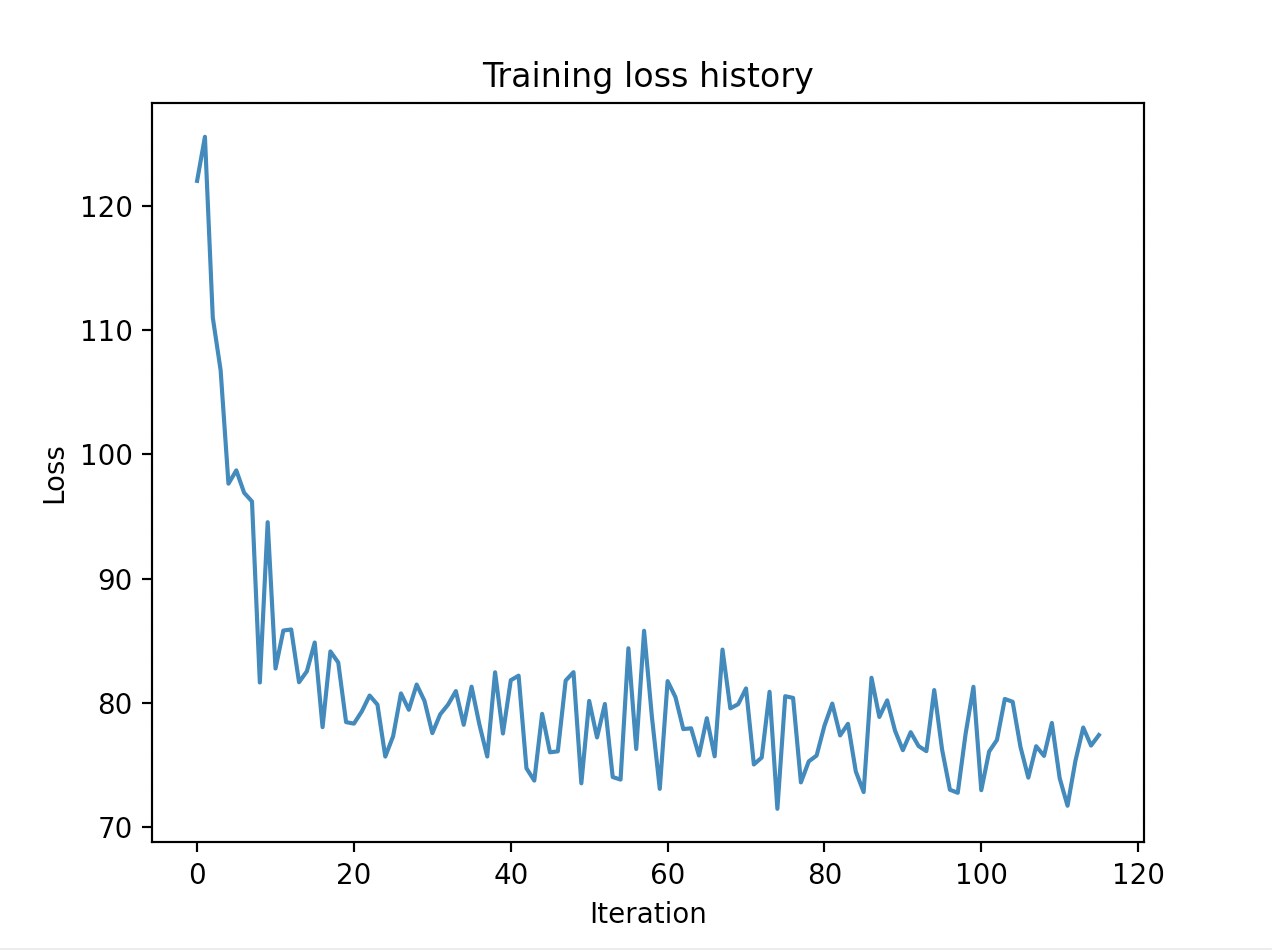
\includegraphics[width=4in,height=3.2in]{rnn} 
        \caption{Training loss history} 
    \end{figure}
    Figure 2 shows the learning curves of training loss.

    \begin{figure}[H]  
        \centering  
        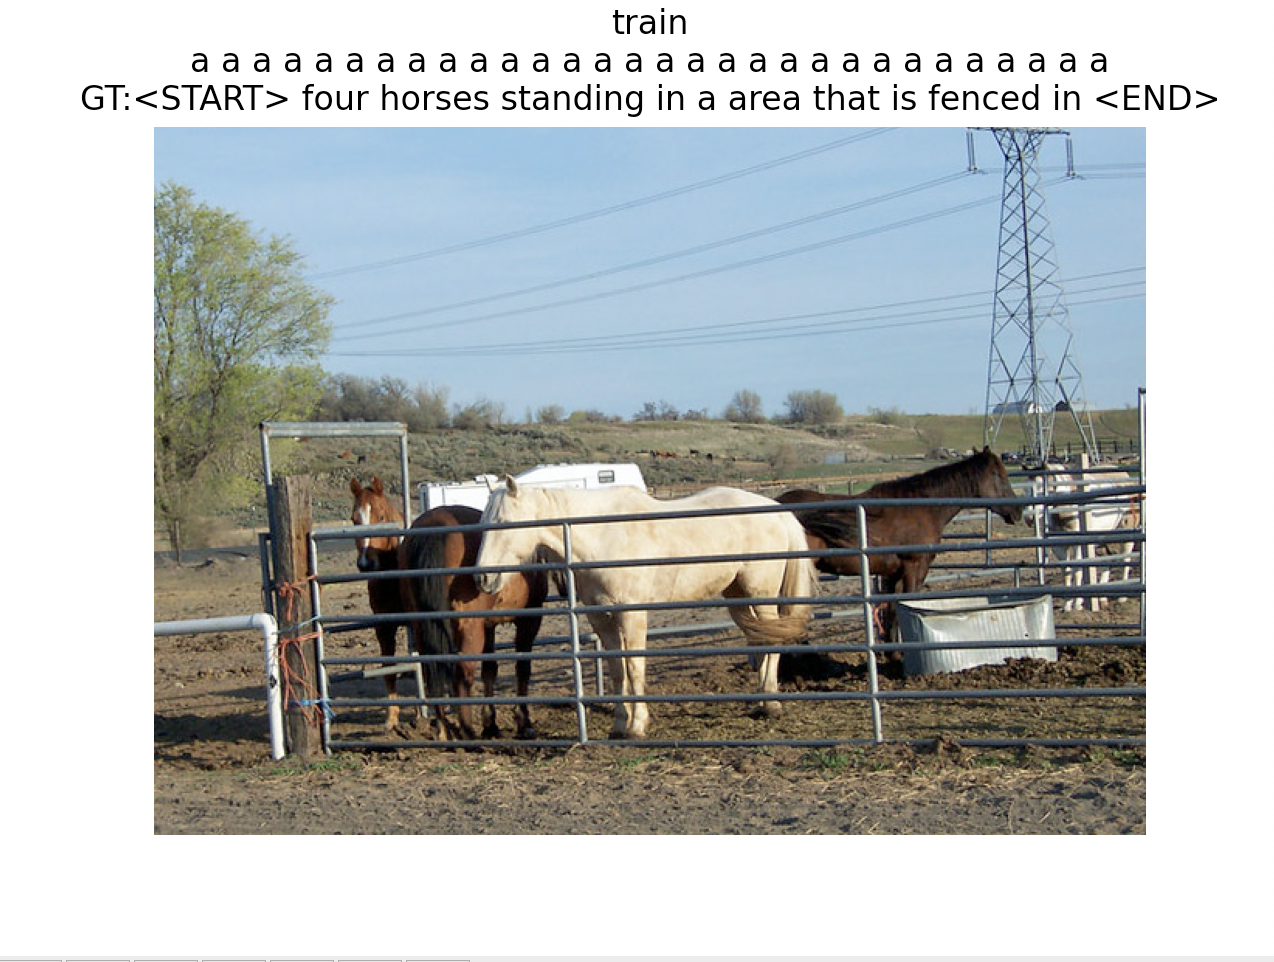
\includegraphics[width=4in,height=3.2in]{cow1} 
        \caption{caption samples of horses} 
    \end{figure}

    \begin{figure}[H]  
        \centering  
        \includegraphics[width=4in,height=3.2in]{train} 
        \caption{caption samples of train} 
    \end{figure}

    \begin{figure}[H]  
        \centering  
        \includegraphics[width=4in,height=3.2in]{surf} 
        \caption{caption samples of surf} 
    \end{figure}

    \begin{figure}[H]  
        \centering  
        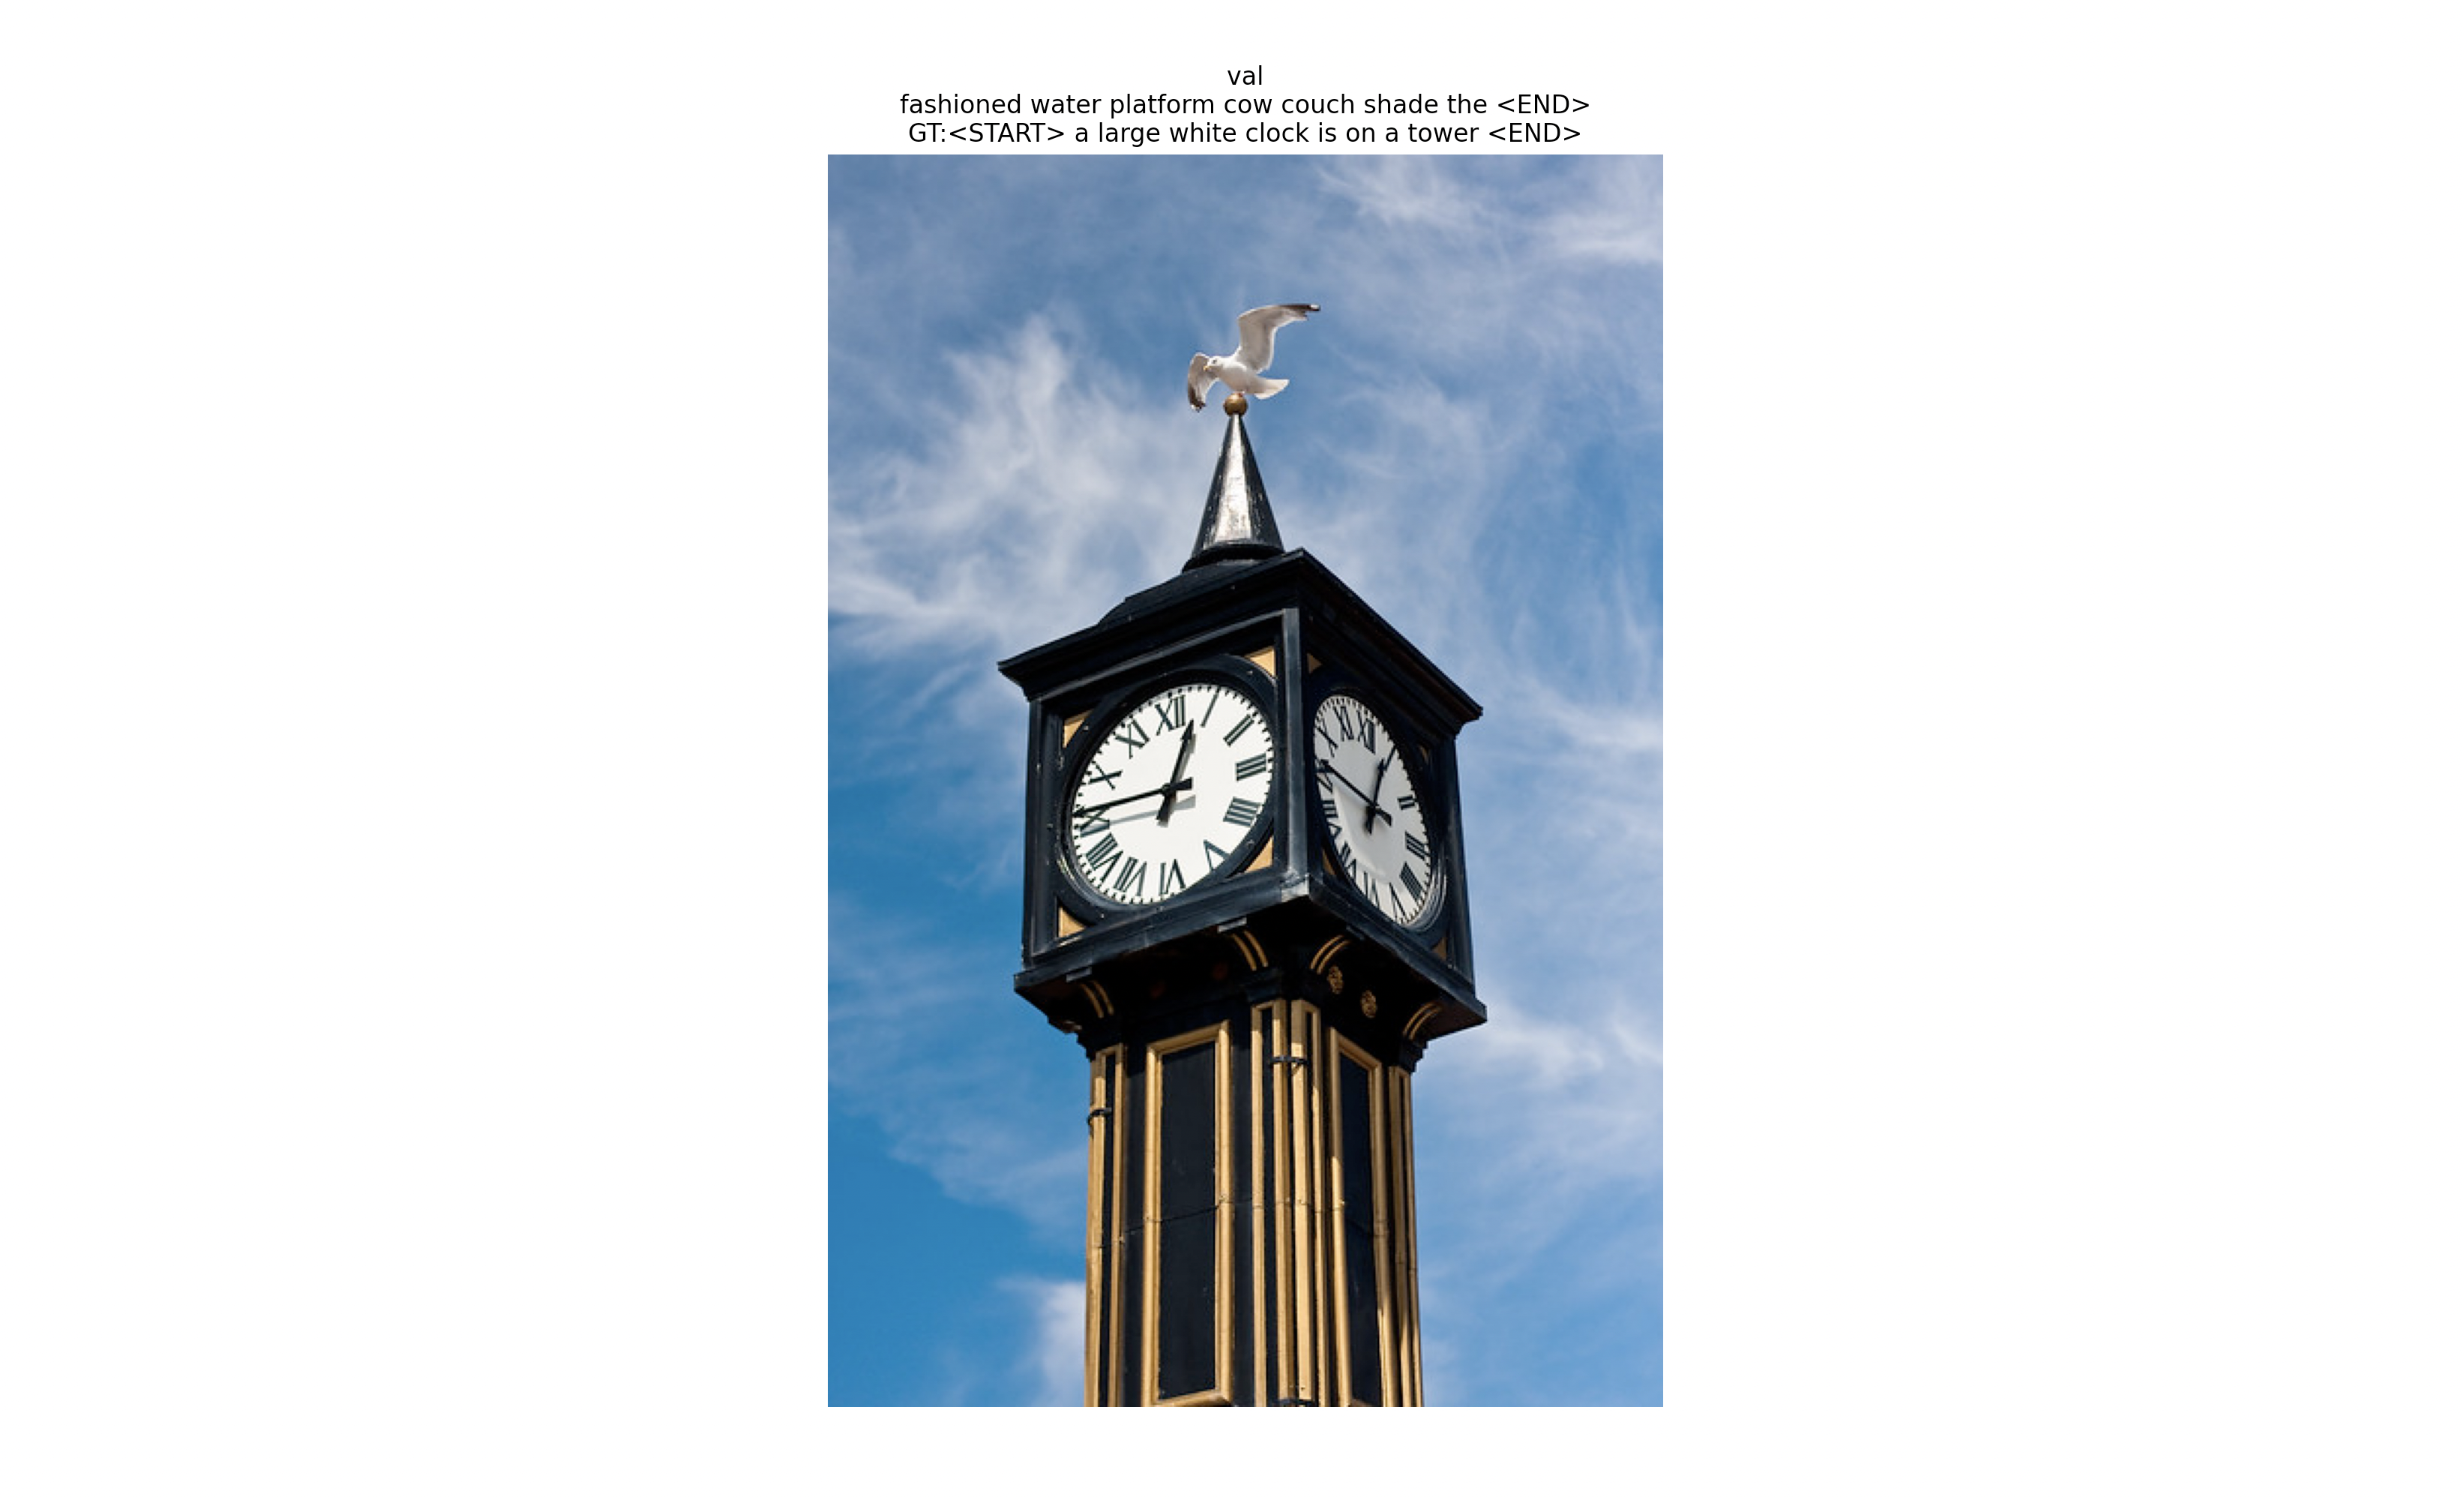
\includegraphics[width=4in,height=3.2in]{tower} 
        \caption{caption samples of tower} 
    \end{figure}
\end{homeworkProblem}
Figure 3, 4, 5, 6 show the caption samples based on my well-trained network.
\pagebreak

\begin{homeworkProblem}
    \large Convolutional Neural Network for multi-class classification\\

    \textbf{Solution}

    \textbf{Part a:}\\

    \textbf{Part b:}\\

    \textbf{Part c:}\\

    \textbf{Part d:}\\

    \textbf{Part e:}\\
    \begin{figure}[H]  
        \centering  
        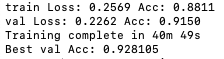
\includegraphics[width=6in,height=3in]{rnn_1} 
        \caption{accuracy on validation dataset} 
    \end{figure}

    \begin{figure}[H]  
        \centering  
        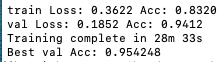
\includegraphics[width=6in,height=3in]{rnn_2} 
        \caption{accuracy on validation dataset} 
    \end{figure}
\end{homeworkProblem}
\pagebreak


\begin{homeworkProblem}
    \large Convolutional Backward Pass
    \newline

    \textbf{Solution}
    \begin{equation}
        \begin{aligned}
            Y_{n, f} &= \sum_{c = 1}^{C} X_{n, c} \ast_{filt} K_{f, c}\\
            Y_{n, f, p, q} &= \sum_{c = 1}^C\sum_{m = 1}^{H''}\sum_{n = 1}^{W''}X_{n, c, p+m-1, q+n-1} \cdot K_{f, c, m, n}\\
            &=\sum_{c = 1}^C\sum_{i = p}^{p+H''-1}\sum_{j = q}^{q+W''-1}X_{n, c, i, j} \cdot K_{f, c, i-p+1, j-q+1}\\
            \Rightarrow \frac{\partial Y_{n, f, p, q}}{\partial X_{n, c, i, j}} &= \sum_{c = 1}^C   K_{f, c, i-p+1, j-q+1}\\
        \end{aligned}
    \end{equation}.\\
    With hint 1,
    \begin{equation}
        \begin{aligned}
            \frac{\partial L}{\partial X_{n, c, i, j}} &= \sum_{f=1}^F\sum_{p=1}^{H^{''}}\sum_{q=1}^{W^{''}}\frac{\partial Y_{n, f, p, q}}{\partial X_{n, c, i, j}}\frac{\partial L}{\partial Y_{n, f, p, q}}\\
            &= \sum_{f=1}^F\sum_{c=1}^C\sum_{p=1}^{H^{''}}\sum_{q=1}^{W^{''}} K_{f, c, i-p+1, j-q+1} \frac{\partial L}{\partial Y_{n, f, p, q}}\\
            &=  \sum_{f=1}^F\sum_{c=1}^C\sum_{m=i}^{i - H^{''} + 1}\sum_{n=j}^{j - W^{''} + 1} K_{f, c, m, n} \frac{\partial L}{\partial Y_{n, f, i-m+1, j-n+1}}\\
            &\Rightarrow \frac{\partial L}{\partial X_{n, c}} = \sum_{f = 1}^F K_{f, c} \ast_{full}(\frac{\partial L}{\partial Y_{n, f}})
        \end{aligned}
    \end{equation}.\\
    Where $m = i - p + 1, n = j -q + 1.$
    \\
    \pagebreak
    \begin{equation}
        \begin{aligned}
            Y_{n, f, p, q} &= \sum_{c = 1}^C\sum_{m = 1}^{H''}\sum_{n = 1}^{W''}X_{n, c, p+m-1, q+n-1} \cdot K_{f, c, m, n}\\
            &=\sum_{c = 1}^C\sum_{i = p}^{p+H''-1}\sum_{j = q}^{q+W''-1}X_{n, c, i, j} \cdot K_{f, c, i-p+1, j-q+1}\\
            \Rightarrow \frac{\partial Y_{n, f, p, q}}{\partial K_{f, c, i, j}} &= \sum_{c = 1}^C   X_{n, c, p+i-1, q+j-1}\\
        \end{aligned}
    \end{equation}.\\
    With hint 2,
    \begin{equation}
        \begin{aligned}
            \frac{\partial L}{\partial K_{f, c, i, j}} &= \sum_{n=1}^N\sum_{p=1}^{H^{''}}\sum_{q=1}^{W^{''}}\sum_{c=1}^C\frac{\partial Y_{n, f, p, q}}{\partial K_{f, c, i, j}}\frac{\partial L}{\partial Y_{n, f, p, q}}\\
            &= \sum_{f=1}^N\sum_{c=1}^C\sum_{p=1}^{H^{''}}\sum_{q=1}^{W^{''}} X_{n, c, p+i-1, q+j-1} \frac{\partial L}{\partial Y_{n, f, p, q}}\\
            &=  \sum_{f=1}^N\sum_{c=1}^C\sum_{m=i}^{i + H^{''} - 1}\sum_{n=j}^{j + W^{''} - 1} X_{n, c, m, n} \frac{\partial L}{\partial Y_{n, f, m-i+1, n-j+1}}\\
            &\Rightarrow \frac{\partial L}{\partial K_{f, c}} = \sum_{n = 1}^N X_{n, c} \ast_{filt}(\frac{\partial L}{\partial Y_{n, f}})
        \end{aligned}
    \end{equation}.\\
    Where $m = p + i - 1, n = q + j - 1.$
    \pagebreak
\end{homeworkProblem}
\end{document}